\section{SECH 2: Static Secret Shared OOB}
The \ac{SECH} 2 design uses only symmetric encryption, and can be deployed either with a long term shared secret, or by using a bootstrapping step to establish the shared secret.

\subsection{Motivations and Deployment Scenarios}

The amount of `cover' available in the TLS 1.3 \ac{CH} message in which we can hide information without differentiating the message from an a normal TLS 1.3 message is limited.
By using only a symmetric encryption algorithm as the basis for sending the stealthy information there is a smaller overhead than for \ac{HPKE}.

While more cover is potentially available we
pursue a design here that leverages only the
\var{random} and \var{legacy\_session\_id} fields,
as explained in Section~\ref{sec:sech-cover-constraints}.

% Other fields/extensions with values that {\em may} look random (and thus might provide cover) are the cipher suite GREASE values, the PSK identity, the \var{key\_share} itself.
% However, the cover provided by these fields/extensions would be less certain because they differ across situations/implementations of TLS. Using these effectively as cover for stealthy bits would involve mimicking the behaviour of a specific implementation in order not to stick out.


% [ ] if the client and server can share the OOB secret securely then we can implement a highly stealthy and cryptographically secure inner SNI
The \ac{AEAD}-only encryption we'll use here
sticks out less than asymmetric encryption.
Asymmetric ciphertexts contain more structure
than symmetric ciphertexts.
With an asymmetric cryptosystem there is
a mathematical relationship between the ciphertext and the private key,
which results in the bytes of the ciphertext being non-uniformly distributed.

% [ ] since the server does not have to publish a public key (as in ECH), it is possible to hide the fact that the server is support SECH from all except the client who knows the OOB secret

% [ ] the secret could be shared amongst multiple clients, allowing for some scale of deployment, but this protocol is certainly not appropriate for internet scale deployments (millions of clients). The more widely the secret is shared the more likely it is to be leaked.
A major challenge with the \ac{AEAD}-only approach
is scaling to multiple users. We could scale by sharing the \varsechlongtermkey{} to
multiple users, but this violates the requirement to `avoid widely shared secrets'.
Another approach would be to enable a distinct \varsechlongtermkey{} for each client-server pair,
but this entails costly trial decryption.
Our preferred approach involves using the \ac{PSK} system to bootstrap a shared secret between the client and client-facing server,
which can be used as the \varsechlongtermkey{}
in a subsequent connection.

This design is {\em not} forward secret in the case of repeated use of the \varsechlongtermkey{}.
However, by repeatedly using the \ac{PSK} bootstrap step we can achieve forward secrecy for the inner servername.

\subsection{Design}

We assume the client and client-facing server have some way to securely share a secret out-of-band; call this secret $s$ or \varsechlongtermkey{}.
The shared secret should be a random string of at least 32 octets, or a longer string with at least that much entropy.

The client wishes to communicate \var{sech\_inner\_servername} and \var{sech\_inner\_alpn} secretly and stealthily to the client-facing server.
The maximum length of the \ac{SECH} payload is \sechtwoservernamelen{}.
The \var{sech\_inner\_servername} is concatenade with \var{sech\_inner\_alpn} (separated by the null byte)
and this is padded
with a suffix of zeros to yield \var{sech\_payload} which is \sechtwoservernamelen{} octets long.
The \var{sech\_inner\_alpn} is optional and may have 0 length.
The client also generates a session-specific \sechtwoivlen{} octet \nonce.
The plain text for encryption $pt$ is the \sechtwoservernamelen{} octet \var{sech\_payload} concatenated with a \sechtworandomlen{} byte inner random.

The session \ac{SECH} 2 encryption key $sk_c$=\var{sech\_session\_secret} is computed as defined in Listing~\ref{lst:sech2-derive-secret}.

The client should ensure that it has never used the $(\nonce,sk_c)$ pair before, but ensuring that $(\nonce,sk_c)$ are never reused globally may not be feasible.
The $(\nonce,sk_c)$ should never be used twice by any clients,
but if there a multiple clients that do not coordinate this will be impossible to guarantee.
However, the fact that $sk_c$ is both secret and fresh
makes it difficult for a attacker to exploit \nonce brittleness. % TODO: move to evaluation

We note that the \var{random} and \varlegacysessionid{} give us 64 octets in which we hide the \ac{SECH} 2 offer, and we call this cover field $c$.
This cover is occupied as depicted in Figure~\ref{fig:sech2-cover}.

To construct \ac{CHO} the client first construct the \ac{CH} as specified RFC 8446,
but stops before computing the \ac{PSK} \var{binders}.
Also bytes \sechtwocipheroffset{} to 64 of $c$ need not be randomly generated,
and bytes 0 to \sechtwocipheroffset{} are replaced with the \ac{AEAD} \nonce.

The \ac{AEAD} encrypted text has length \sechtwocipherlen{} and is placed in bytes \sechtwocipheroffset{}  to \sechtwocipherend{} of $c$, as depicted in Figure~\ref{fig:sech2-cover}.

% At last the \ac{PSK} \var{binders} are computed, if necessary, yielding the \ac{CHO}.

We define \var{ClientHelloOuterAAD} as a clone of \var{ClientHelloOuter}, except with bytes 12 to 64 of the cover $c$ set to 0s, and if the \var{pre\_shared\_key} extension is present then the \var{binders} field is set to all 0s.
The session key $sk_c$ can only be computed after \var{Client\-HelloOuterAAD} is known.
The secure derivation of $sk_c$ depends on the entropy of the \var{key\_share} extension and/or the \ac{PSK} identity included in \var{ClientHelloOuterAAD}.
An example transcript of a \var{ClientHelloOuterAAD} can be seen in Listing~\ref{lst:client-hello-outer-aad-example-sech2}.

\begin{listing}[H]
\centering
\fbox{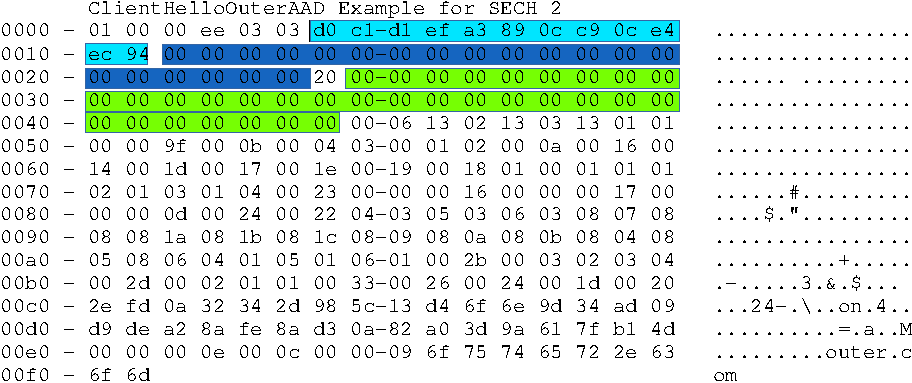
\includegraphics[width=\linewidth]{figure-static/choaad-sech2-example.pdf}}
\captionsetup{width=.8\linewidth} 
\caption[SECH 2 \var{ClientHelloOuterAAD} Example]{An example transcript of the \var{ClientHelloOuterAAD} for \ac{SECH} 2. Light blue: \ac{AEAD} nonce (first 12 bytes of \var{random}). Dark blue: remainder of \var{random} set to 0. Green: \varlegacysessionid{} set to 0.
The left column shows the index of the of the first byte in row in hexadecimal. The middle column shows the actual values in hexadecimal, and the rightmost column shows an ASCII rendering of the values. Rows \var{0x00c0} and \var{0x00d0} contain the 32 bytes of an \ac{X25519} public value.}
\label{lst:client-hello-outer-aad-example-sech2}
\end{listing}


% [] ] TODO: what if key\_share is not included, e.g. for PSK-only handshake? Reject SECH?

%the transcript of \var{ClientHelloInner} message, which is \var{ClientHelloOuter} but with: 1. the encrypted AEAD output replaced with the plain text \var{sech\_inner\_servername} and \var{sech\_inner\_random}, as well as 2. the \var{extension\_data} field of the \var{server\_name} extension set to all 0s with the same length as the cover value for \var{server\_name} (The backend server does not learn the cover SNI used). The AEAD MAC $t$ is left in \var{ClientHelloInner}.

\begin{listing}[htb]
\centering
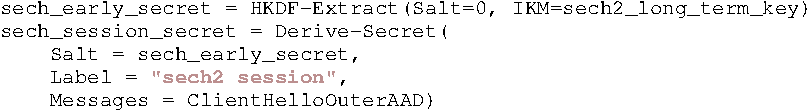
\includegraphics[width=\linewidth]{figure/sech2-derive-secret.pdf}
\captionsetup{width=.8\linewidth} 
\caption[SECH 2 Derive Secret]{Derive $sk_c$, the secret key that will be used by the client to encrypt $pt$ which has the inner \var{CH} data.}
\label{lst:sech2-derive-secret}
\end{listing}

The client encrypts $pt$ (authenticating $aad$) with $(\nonce,sk_c)$ using AES-128-GCM, producing a \sechtwotaglen{} octet authentication tag $t$ and the \sechtwocipherlen{} octet encrypted text $ct$. The \ac{CHO} has $c:=\nonce||ct||t$. The placement of the required values in cover $c$ of the \ac{CHO} is depicted in Figure~\ref{fig:sech2-cover}.
Finally the \ac{PSK} \var{binders} are inserted, which digest the \nonce, $ct$, and $t$.

\begin{figure}[htb]
\centering
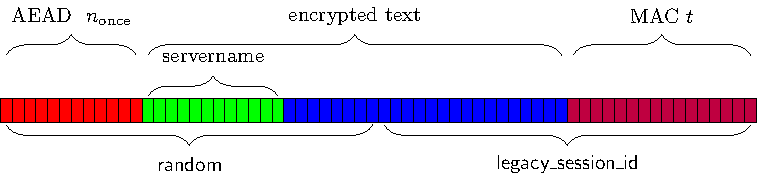
\includegraphics[width=\linewidth]{figure/sech2-cover.pdf}
\captionsetup{width=.8\linewidth} 
\caption[SECH 2 Cover]{Locations of AEAD inputs and outputs in the 64 octets of \ac{CH}\var{.random} and \ac{CH}\var{.legacy\_session\_id}. The cipher text $ct$ and MAC tag $t$ outputs are a function of $iv$, $sk_c$, $pt$, and $aad$: $(ct,t)=\text{AEAD}(iv,sk_c,pt,aad)$.}
\label{fig:sech2-cover}
\end{figure}

A cooperating server in possession of \varsechlongtermkey{} that receives a \ac{CH}
first constructs \var{ClientHelloOuterAAD}, then $sk_c$,
and attempts to decrypt and authenticate $ct$.
If decryption/authentication are unsuccessful the server continues with the \ac{TLS} 1.3 handshake as normal.
If successful, the client-facing server forwards \ac{CHI} to the backend server identified by the inner server name.
If the inner server name does not identify a backend server then the client-facing server continues the \ac{TLS} 1.3 handshake as if \ac{SECH} 2 is disabled.

The \ac{CHI} message  is a clone of \ac{CHO} but with:
1. the encrypted AEAD output $ct$ replaced with the plain text $pt$, as well as
2. the \var{extension\_data} field of the \var{server\_name} extension set to all 0s with the same length as the cover value for \var{server\_name} (The backend server does not learn the cover \ac{SNI} used).
The \ac{AEAD} \nonce and \ac{MAC} $t$ are left in \var{ClientHelloInner}.

The backend server can distinguish a \ac{CHI}
from a regular \ac{CH} by the \var{server\_name} extension.
If the \var{extension\_data} field of the \var{server\_name} has all 0s it is treated as a \var{ClientHelloInner}.
Otherwise it should be treated as a regular \ac{TLS} 1.3 \ac{CH}.
Note that if an attacker can send \ac{CH} directly to
the backend server,
then the client's reaction to an all zero \ac{SNI} can break
channel-level \ac{PC}.
For this reason the backend server must only process messages
from the client-facing server as \ac{CHI}s.
Authentication of the client-facing server is beyond the scope of this specification.
Also, a server tha receives a \ac{CH} whose \ac{SNI} is all 0s must abort with an appropriate alert. % TODO: how do clients typically react to an all zero \ac{SNI}

The server parses the plaintext $pt$
to retrieve the inner server name and inner \ac{ALPN} list
(if present)
in order to select an identity.
At this point the backend server might respond with \var{HRR} or \var{ServerHello}.
As discussed in Section~\ref{sec:hrr-hijacking} in the case of a \var{HRR}
the client and server essentially abandon the attempt to complete the \ac{SECH}
handshake successfully and craft the remaining messages solely for the purpose
of maintaining stealth.
This means the server should select an identity corresponding to the outer \ac{SNI}.
This can be achieved easily in shared-mode, but not split-mode,
since in split-mode the backend server for the outer \ac{SNI}
will not have seen the \ac{CH} or \ac{HRR} messages
needed for the transcript.
It is for this reason that our design of \ac{SECH} 2 does not work in split-mode.

%If the server accepts the first \ac{CHO}
%\ac{SECH} can proceed.
%Whereas in \ac{ECH} the acceptance signal is always sent in the server's first message
%(whether it is a \var{HRR} or \var{SH}),
%for \ac{SECH} 2 the acceptance signal is always in the \var{SH}.
%The client-facing server forwards these (and subsequent) messages to the client unaltered.
If the backend server accepts the parameters of \ac{CHI}
and accepts the inner servername identified in $pt$,
then it responds with a special \ac{SH} containing an \ac{SECH} acceptance signal.
Also, if using certificate-based authentication, then the later \ac{tlsC} message should contain a certificate identified by $pt$.

\begin{listing}[H]
\centering
\fbox{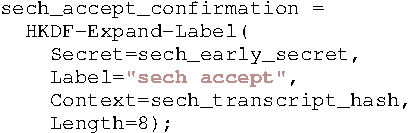
\includegraphics[width=.7\linewidth]{figure/sech2-accept-function.pdf}}
\captionsetup{width=.8\linewidth} 
\caption[SECH 2 Accept Confirmation]{The function used to calculate the SECH 2 acceptance signal using the \var{HKDF-Expand-Label} function defined in Section 7.1 of RFC 8446 (\cite{rfc8446}). The \var{sech\_early\_secret} is derived from $s$ as defined in Listing~\ref{lst:sech2-derive-secret}, and \var{sech\_transcript\_hash} is described in Listing~\ref{lst:sech2-transcript-hash}.}
\label{lst:sech2-accept-function}
\end{listing}

The \ac{SECH} 2 acceptance signal is 24 octets long and placed in the first 24 bytes of the \ac{SH}\var{.random},
such that it does not overlap with the \ac{ECH} acceptance signal.
It is a function of a hash of the transcript of the handshake so far, \varsechtranscripthash{},
and $s=$\varsechlongtermkey{}.
We define \varsechacceptconfirmation{} in Listing~\ref{lst:sech2-accept-function} and \varsechtranscripthash{} in Listing~\ref{lst:sech2-transcript-hash}.

\begin{listing}[H]

\centering
\fbox{
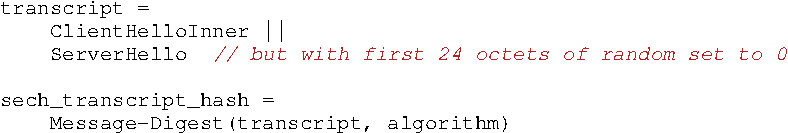
\includegraphics[width=\linewidth]{figure/sech2-transcript-hash.pdf}}
\captionsetup{width=.8\linewidth} 
\caption[SECH 2 Transcript Hash]{Specification of the \var{sech\_transcript\_hash} used to calculate \var{sech\_accept\_confirmation}. The \var{algorithm} is the hash algorithm of the negotiated cipher suite for the handshake. Blue: the decrypted inner servername padded to 12 bytes. Green: the location of the acceptance confirmation set to 0.}
\label{lst:sech2-transcript-hash}

\end{listing}

\begin{listing}[htb]

\centering
\fbox{
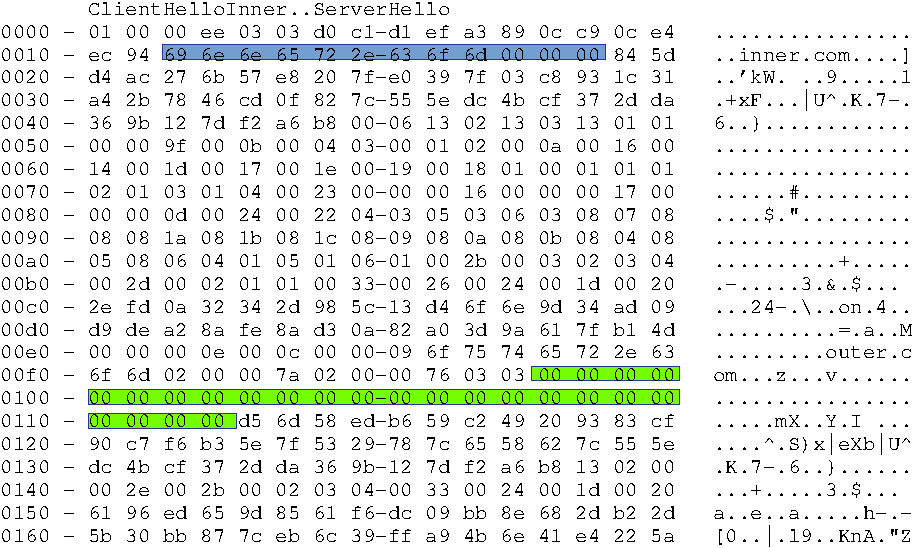
\includegraphics[width=\linewidth]{figure-static/chi-sh-sech2-example.pdf}}
\captionsetup{width=0.8\linewidth} 
\caption[SECH 2 Transcript Example]{An example transcript of \ac{CHI} concatenated with the \ac{SH}, i.e. the value of \var{transcript} defined in Listing~\ref{lst:sech2-transcript-hash}.}
\label{lst:sech2-transcript-hash-example}

\end{listing}

% The client uses that secret to encrypt the true target servername as well as a 32 byte secret inner nonce which are hidden in the ClientHello \var{random} and the \var{pre\_shared\_key} extension. The inclusion of the secret inner nonce is necessary to mitigate cut-and-paste attacks.

% More precisely, the client generates a 12 byte initialisation vector for AES-128-GCM. The plaintext is an ASCII encoding of the servername padded with 0x00 up to 12 bytes, appended to the 32 byte inner nonce.
% AEAD is used but the AAD is 0-length. % TODO: might be better to use the transcript hash of ClientHello (with random zeroed) as AAD, (however, if random is zeroed then transcript hash might not change)
% The AEAD tag is truncated to 8 bytes, such that we have a combined 64 bytes to send, which are put into the \var{ClientHello.random} and \var{ClientHello.legacy\_session\_id}. The first 12 bytes contain the IV, the next 12 contain the first 12 bytes of the cipher text, and the last 8 bytes of the \var{random} contain the truncated MAC, and the \var{ClientHello.legacy\_session\_id} is the last 

If the backend server accepts SECH 2 then it makes the SECH inner servername available to the application program via a callback or some other means, which allows the application program to decide whether or not to switch contexts (server certificate etc.).

The remainder of the handshake is carried out as in RFC 8446,
using the \ac{CHI} instead of \ac{CHO} for the transcript.

\subsection{Distributing SECH 2 Access}
Here we describe a mechanism for accessing an \ac{SECH} 2 server
without each client needing to know the \varsechlongtermkey{}.

A resumption \ac{PSK} (advertised via an \ac{NST})
is bound cryptographically to the transcript of the first handshake as well as most of the \var{CH} for the second handshake.
The binding to the first handshake arises because the \ac{PSK} is derived from the key schedule
of the first handshake.
The binding to the second handshake is achieved using a \ac{HMAC} called the \var{binder}.
Pseudo-code for the construction of the \var{binder} value is presented in Listing~\ref{lst:binder-pseudocode}.

\begin{listing}
    \begin{Verbatim}[frame=single]
early_secret = HKDF-Extract(0, PSK)
binder_key = Derive-Secret(early_secret, "res binder", "")
binder_finished_key = HKDF-Expand-Label(
    binder_key,
    "finished",
    "",
    Hash.length)
binder =
    HMAC(binder_finished_key,
        Transcript-Hash(Truncate(ClientHello)))
    \end{Verbatim}
    \captionsetup{width=.8\linewidth} 
    \caption[Pseudo-code for Computation of  \var{binder}]{\label{lst:binder-pseudocode}Pseudo-code of the process used to compute a \var{binder} when using a resumption PSK. \ac{CH} is truncated so as not to include the \var{binders} list itself. We'll tweak this formulation slightly in the case of \ac{SECH} 2.}
\end{listing}


% [ ] TODO research has anyone done ticket sharing amongst clients before? E.g. client with multiple processes

% [ ] TODO bleichenbacher attack

Sharing the \ac{SECH} 2 long term secret widely amongst clients would violate the `Avoid Widely Shared Secrets' requirement advocated by \citep{rfc8744-issues}.
How do we facilitate connections from large numbers of clients while restricting each long term secret to being shared to only 2 parties?
One option is to have a distinct long term secret for each client-server pair.
The \ac{SECH} 2 design specified here can facilitate this through trial decryption,
i.e. every \ac{CHO} processed by the server
is checked against each registered secret
until one is found to successfully decrypt the inner server name.
This approach scales horribly,
with the cost of every connection being proportional to the number of registered clients,
whether or not those clients are active.
But note that this trial decryption process is highly parallelizable.

Our approach to distributing access to the \ac{SECH} 2 capability
exploits \ac{PSK}s,
either via gossiping or bootstrapping.
The first step is for a client C1 to establish a resumption \ac{PSK} with
the client-facing server.
For the bootstrap approach: in a subsequent connection the client can use this \ac{PSK}
as if it were the \varsechlongtermkey{}, while also supplying
the \ac{PSK} identity in the \ac{PSK} extension.
Similarly for the gossiping approach C1 passes the \ac{PSK} (and associated identity)
to another client C2, and C2 uses this \ac{PSK} to perform \ac{SECH} 2.
The backend server will not recognise the \ac{PSK} identity and ignores it.

In split-mode, the initial bootstrap connection is with the client-facing server, whereas
the \ac{SECH} 2 conneciton is with the backend server. This means the second connection
cannot itself be used to establish \ac{PSK}s for subsequent connections.
The bootstrap connection yields some number $n$ of \ac{PSK}s that can be used for connecting
to the backend server, but once these \ac{PSK}s are expended the bootstrap step has to be repeated.
In shared-mode, however, \ac{PSK}s established with the backend server can be used
for subsequent \ac{SECH} 2 connections.